\documentclass{article}
\usepackage[utf8]{inputenc}
\usepackage{amssymb}
\usepackage{tikz}
\usepackage{amsmath}
\usepackage{relsize}
\usepackage{mathtools}
\usepackage{textcomp}
\usepackage{eurosym}
\usepackage{amssymb}
\usepackage{systeme}
\usepackage{mathtools}
\usepackage{todonotes}
\usepackage[autopunct=true]{csquotes}
\title{Results}
\author{Roman Oort}
\date{\today}

%%% PERSONAL SHORTCUTS
\DeclareMathOperator*{\plim}{plim}
\newcommand{\T}{\textbf{T}}
\newcommand{\Tij}{\textbf{T}_{ij}}
\newcommand{\Soc}{(\T(n))^{\infty}_{n=1}}
\newcommand{\beli}[3][2]{p_{#2}^{(#3)}}
\newcommand{\belvec}[2]{\textbf{p}^{(#2)}}

\begin{document}

\maketitle

\tableofcontents
\newpage
\section{Results}
\label{results}

The results following in this section are all obtained from networks randomly generated using the same parameters. More specifically, every generated network is a directed network with an increased degree, where each agent is guaranteed to have self-link. For generating the additional degree the default distribution, as seen in Section [REF] is used.

\noindent Furthermore, the results shown for the standard deviation, distance from the assumed truth and the convergence time, are averaged over ten iterations, in order to obtain a more general view. For each of the iterations a new network and initial belief vector was generated, using the same parameters as mentioned above. The graph that shows the convergence of the network towards the truth of the model is simply taken to be the last of these ten iterations.

\noindent Finally, not every updating rule showed uniform convergence. That is to say, that it was not the case that for every updating rule the agents will all adopt the same belief at the time of convergence. Whenever it was the case that the standard deviation of the belief vector at the time of convergence did not equal $0$, the convergent belief was taken to be the mean of the belief vector.

\subsection{Cooperative Networks}

As can be seen in Figure \ref{coop:compare}, in a cooperative network all updating rule behave quite similar. The convergent belief differs the most for smaller network. However, as the network size increases this difference dissipates, and the convergent beliefs become more and more similar, both to the other updating rules \emph{and} the assumed truth of the model.

\noindent However, while the convergent beliefs are mostly similar, the standard deviation of the convergent belief vector does differ significantly between updating rules. Where the regular and thresholded DeGroot mechanics have no deviation in the convergent belief vector, meaning they have a uniform convergent belief held by every agent, the other updating rules end up with a non-insignificant amount of variation in the belief vector. This means that, at the time of convergence, it is not the case that the different agents all hold the same beliefs, but rather, while their opinions may not change anymore, they still hold different opinions. 

\noindent Finally, the thresholded and regular DeGroot mechanics both reach convergence in the same amount of time, while the other updating rules are significantly faster to reach the point of convergence.

\begin{center}
    \begin{figure}[!htbp]
        \centering
        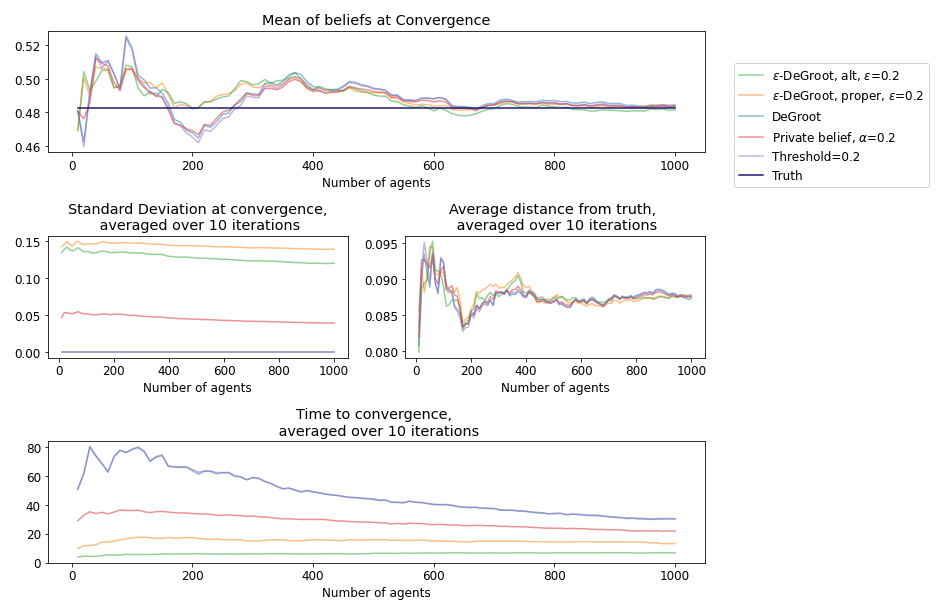
\includegraphics[width=1.2\textwidth]{ThesisKI/Images/WisdomCompare0.png}
        \caption{Convergence Behaviour Threshold Updating}
        \label{coop:compare}
    \end{figure}
\end{center}

\newpage

\subsection{Non-cooperative networks, $n=1$}

Where the different updating rules behaved in a similar fashion as the regular DeGroot updating mechanics in a fully cooperative network, significant differences occur when applied to a network with even one non-cooperative agent, as demonstrated in Figure \ref{noncoop1:compare}. 

\noindent First of all, as expected, under regular DeGroot dynamics the convergent opinion becomes that of the non-cooperative agent, and the same goes for the thresholded DeGroot mechanics. Furthermore, again as expected, this belief is held by every agent in the network, which is expressed by the $0$ standard deviation of the convergent belief vector of these updating rules. However, the other three updating mechanics exhibit vastly different behaviour. Instead of converging towards the opinion of the non-cooperative agent, the network still converges towards the truth. However, once again, this is not a uniform convergence, as there still is some standard deviation in the convergent belief vector, though this appears to decline ever so slightly as the network size increases. However, the standard deviation for the private belief updating rule is somewhat higher when compared to a fully cooperative network Figure \ref{coop:compare}.

\noindent Finally, the updating time for both the regular and the thresholded DeGroot mechanics behave nearly identical, and both display a significant increase in convergence time, whereas the other three updating rules do not appear to show significantly slower convergence. This increase in convergence time can be explained by the presence of the single non-cooperative agent, whose influence has to spread throughout the entire network, taking more and more time to reach every agent as the network size increases. Furthermore, this appears to be a non-factor for the other updating rules, where the non-cooperative agent is not nearly as formative, or even at all, for the convergent opinion, making it so that it will not significantly impact the convergence time as a result.

\begin{center}
    \begin{figure}[!htbp]
        \centering
        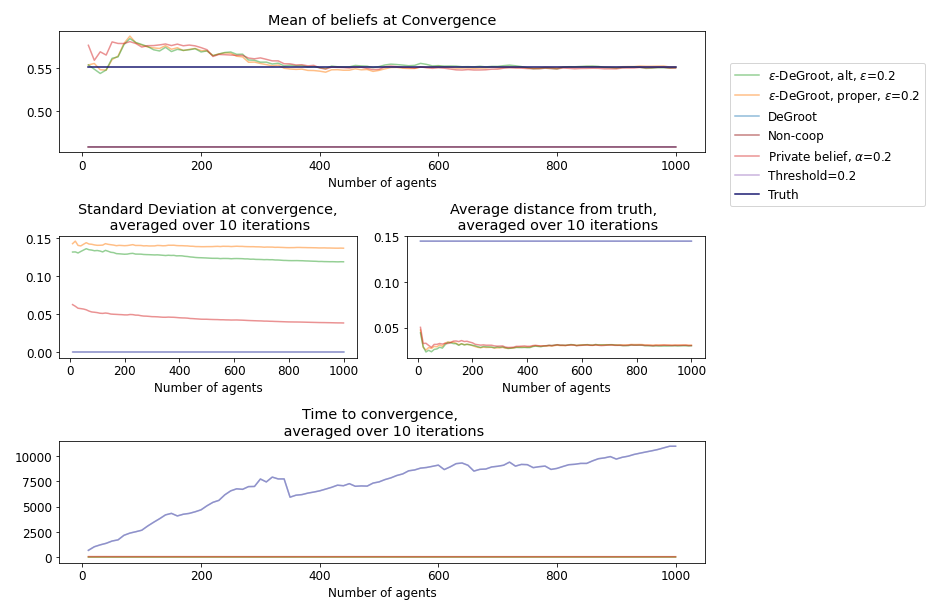
\includegraphics[width=1.2\textwidth]{ThesisKI/Images/WisdomCompare1.png}
        \caption{Convergence Behaviour Non-cooperative Network, $n=1$}
        \label{noncoop1:compare}
    \end{figure}
\end{center}

\newpage

\subsection{Non-cooperative networks, $n > 1$}

Finally, in networks with multiple non-cooperative agents there is once again a significant difference in the behaviour of the various updating rules, as seen in Figure \ref{noncoop+:compare}. Once again, both the regular and thresholded DeGroot mechanics converge towards the opinions of the non-cooperative agents. Tending towards some, weighted, average between the opinions of those agents, even if this average differs from the truth. However, the effect of these non-cooperative agents is negligible to the convergent belief of the network when using the other three updating rules, all of which still converge towards the assumed truth of the network. 

\noindent However, the regualar and thresholded DeGroot mechanic, no longer display this uniform convergence in the presence of multiple non-cooperative agents, although the standard deviation of the convergent belief vector does decrease quickly as the network size increases. On the other hand, the standard deviation of the private belief updating rule appears somewhat higher in the presence of multiple non-cooperative agents, though the slight decrease as the network size increases is still present. The standard deviation of both variations of the $\varepsilon$-DeGroot mechanics behave the same as in the presence of only one non-cooperative agent.

\noindent Finally, while still significantly higher than in the presence of no non-cooperative agents, is shorter than in the presence of only one non-cooperative agent, for both the regular and thresholded DeGroot mechanics. All other three updating rules are still unaffected in their convergence time, as the influence of the non-cooperative agents on their updating process is very limited.

\begin{center}
    \begin{figure}[!htbp]
        \centering
        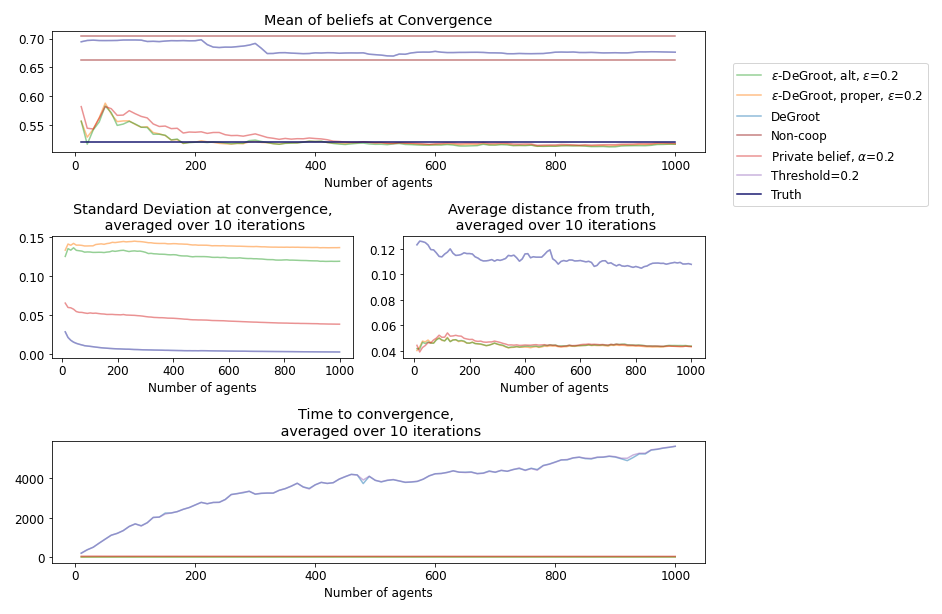
\includegraphics[width=1.2\textwidth]{ThesisKI/Images/WisdomCompare2.png}
        \caption{Convergence Behaviour Non-cooperative Network, $n>1$}
        \label{noncoop+:compare}
    \end{figure}
\end{center}

\newpage

\section{Conclusion}

The goal of the thesis was to examine the behaviour of social networks where agents update their opinions using the DeGroot mechanics, as discussed in Section [REF], and the emergent \emph{Wisdom of Crowds} effect that arises from this updating rule. More specifically, the goal was to examine the influence of any non-cooperative agents, those who refuse to change their opinion, on the \emph{Widsom of Crowds} effect, and which variations of this updating rule could provide a more robust updating rule, more resilient to non-cooperative agents in the network. Five variations on the DeGroot mechanics, described in more detail in Section [REF], were implemented and compared in three different variations of networks; fully cooperative networks, where every agent changes their opinion; non-cooperative networks where there is only one single agent who does not change its opinion; and finally non-cooperative networks with multiple non-cooperative agents. 

\noindent As shown in Section [REF], when the network is fully cooperative the updating rules behave largely similar, all displaying the \emph{Wisdom of Crowds} effect as the network size increases. However, where the regular and thresholded DeGroot mechanics achieve a uniform converge, where every agent holds the same belief at the time of converge, both variations of the $\varepsilon$-DeGroot mechanics and the private belief updating rules do not. Instead of a single convergent belief held by every agent each agent's convergent belief is somewhat different from its neighbours'. However, their average belief still approaches the assumed truth as the network size increases, still achieving the \emph{Wisdom of Crowds} effect, though a somewhat less powerful notion than the regular DeGroot mechanics. Furthermore, the standard deviation of the private belief updating rule is significantly less than that of the $\varepsilon$-DeGroot variations.

\noindent However, strong differences occur when even a single non-cooperative agent is added to the network. Where the regular and thresholded DeGroot mechanics clearly displayed the \emph{Wisdom of Crowds} effect in a cooperative network, this effect is now completely lost. Instead, each individual agent now assumes the opinion of the single non-cooperative agent at the time of convergence. However, this is where the other updating rules separate themselves. While they still do not achieve uniform convergence, though the variation in final opinions decreases somewhat as the network grows, the average of their belief vector at the time of convergence does not equal the belief of the non-cooperative agent. Rather, the \emph{Wisdom of Crowds} effect is still fully present, as the average of the convergent belief vector comes ever closer to the assumed truth, as the network size increases.

\noindent Finally, in the presence of multiple non-cooperative agents, similar results are achieved. Once again, the regular and thresholded DeGroot mechanics tend towards the opinions of the non-cooperative agents, although uniform convergence is no longer achieved, whereas the other updating rules still exhibit the \emph{Wisdom of Crowds} effect. However, instead of one constant belief for the regular and thresholded DeGroot mechanics, the convergent belief seems to vary between different values of $t$, towards some weighted average of the opinion of the non-cooperative agents in the network. Furthermore, in the presence of multiple non-cooperative agents the thresholded DeGroot mechanics also no longer attain uniform convergence, though the standard deviation does clearly tend towards $0$ as the network grows. The other three updating rules however, behave similarly in the presence of multiple non-cooperative agents, still displaying the \emph{Wisdom of Crowds} effect, while the opinions of individual agents do still vary.

\noindent All in all, the $\varepsilon$-DeGroot variations and private belief updating mechanics are successful in making social networks more resilient to the presence of non-cooperative agents, where the thresholded DeGroot mechanics fall short and agents still end up adopting the opinions of the non-cooperative agents. However, these methods are not infallible, as they lose a powerful effect exhibited by the standard DeGroot mechanics. Namely, while these updating rules still converge, it is no longer the case that every agent ends up holding the same opinion, but rather, each agent has a somewhat different opinion from the others.

\section{Future Work}

While interesting results have come forward in this thesis there is still room for improvement, as it would be desirable to find a variation on the updating rule which would still allow for increased resilience towards non-cooperative agents provided by the $\varepsilon$-DeGroot variations and the private belief updating rule, while still allowing for uniform convergence.

\noindent One untested variation of the DeGroot mechanics would allow the weights of the network to vary over time, which has been discussed in \cite{chatterjee1977stochastic}. One of the criticisms of the DeGroot model are its rigid weights, which do not change over time. Therefore a variation of the model where the agent can change the weight they place on others' opinions could be a more accurate reflection of the way people change their opinions, and may provide more resilience in the face non-cooperative agents.

\noindent Furthermore, another way to combat the presence of non-cooperative agents would be to use \textquote{counter non-cooperative agents}. That is to say, non-cooperative agents specifically designed to oppose the already present non-cooperative agents in the network. The information spread by these two kinds of non-cooperative agents could counteract each other allowing the regular cooperative agents to converge towards a common opinion, and eventually the assumed truth, as the network grows sufficiently large.

\noindent Besides examining different updating rules there is also the option to look at different ways that misinformation is spread throughout a network. Another vulnerability of the \emph{Wisdom of Crowds} effect besides the non-cooperative agents is what \cite{amir2021robust} describe as \emph{distorted monitoring}, where every agents' initial signal is shifted over by some amount $\delta$ from the assumed truth, which can simply be implemented by using a non-zero-mean noise signal when generating the initial beliefs.

\noindent Finally, another possible direction for future work is to examine different variations of the non-cooperative agents. Where they are now represented as agents in the network receiving information from no agents but themselves, several alternatives could also be examined. First of all, a possible variation would be to represent the non-cooperative agents as a periodic influence, rather than a permanent addition to the network. Rather than permanently spreading their own opinion to their neighbours they would only spread this information every set amount of time, either to specific agents or to the network at large. 

\noindent Another natural extension of the non-cooperative agents would be to look at groups of non-cooperative agents, where the agents in this group would only receive information from other in this group while still sending information to other agents outside the group.

\bibliographystyle{apalike}
\bibliography{references.bib}

\end{document}